%Autor: miguev
\documentclass[a3paper,12pt]{article}
\usepackage[utf8x]{inputenc}
\usepackage[spanish]{babel}
\usepackage{multicol}
\usepackage{multirow}
\usepackage{eurosym}
\usepackage{graphicx}
\usepackage{fancybox}
\usepackage{color}

% sacado de /usr/share/doc/texmf/latex/geometry/geometry.dvi.gz
% para definir tipo de hoja y márgenes (90% texto, 5% margen izqdo, 5 drcho)
\usepackage[verbose,noheadfoot,dvips,a3paper,hscale=1,vscale=1]{geometry}

\setlength{\hoffset}{5mm}
\setlength{\voffset}{2mm}
\setlength{\textwidth}{297mm}
\setlength{\textheight}{420mm}

\begin{document}
%\begin{tabular}{c}
\rotatebox{90}{
\includegraphics[height=25cm]{cubierta/portada.eps}}% \\


\includegraphics[width=25cm]{cubierta/lomo.eps}% \\

\rotatebox{90}{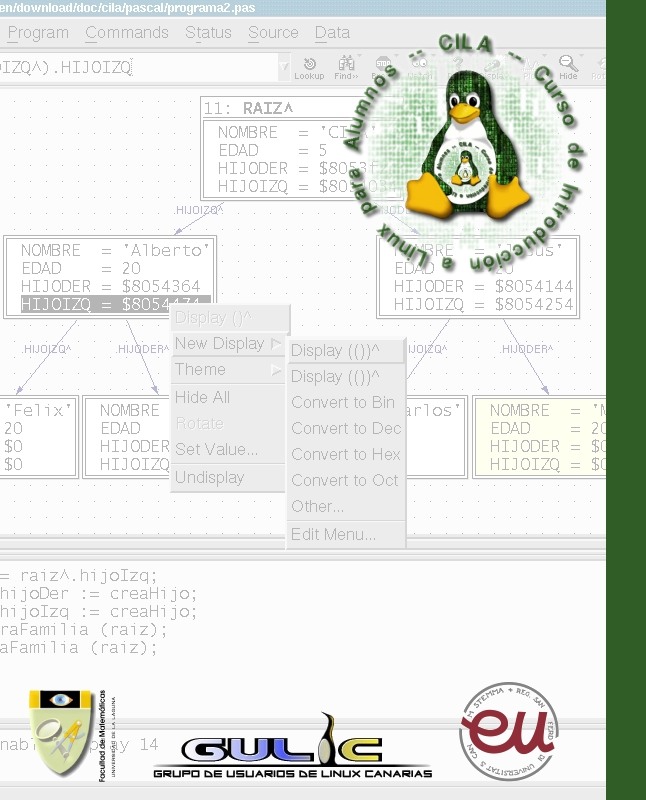
\includegraphics[height=25cm]{cubierta/contraportada.eps}}% \\
%\end{tabular}
\end{document}
